
%% bare_jrnl_compsoc.tex
%% V1.4a
%% 2014/09/17
%% by Michael Shell
%% See:
%% http://www.michaelshell.org/
%% for current contact information.
%%
%% This is a skeleton file demonstrating the use of IEEEtran.cls
%% (requires IEEEtran.cls version 1.8a or later) with an IEEE
%% Computer Society journal paper.
%%
%% Support sites:
%% http://www.michaelshell.org/tex/ieeetran/
%% http://www.ctan.org/tex-archive/macros/latex/contrib/IEEEtran/
%% and
%% http://www.ieee.org/

%%*************************************************************************
%% Legal Notice:
%% This code is offered as-is without any warranty either expressed or
%% implied; without even the implied warranty of MERCHANTABILITY or
%% FITNESS FOR A PARTICULAR PURPOSE! 
%% User assumes all risk.
%% In no event shall IEEE or any contributor to this code be liable for
%% any damages or losses, including, but not limited to, incidental,
%% consequential, or any other damages, resulting from the use or misuse
%% of any information contained here.
%%
%% All comments are the opinions of their respective authors and are not
%% necessarily endorsed by the IEEE.
%%
%% This work is distributed under the LaTeX Project Public License (LPPL)
%% ( http://www.latex-project.org/ ) version 1.3, and may be freely used,
%% distributed and modified. A copy of the LPPL, version 1.3, is included
%% in the base LaTeX documentation of all distributions of LaTeX released
%% 2003/12/01 or later.
%% Retain all contribution notices and credits.
%% ** Modified files should be clearly indicated as such, including  **
%% ** renaming them and changing author support contact information. **
%%
%% File list of work: IEEEtran.cls, IEEEtran_HOWTO.pdf, bare_adv.tex,
%%                    bare_conf.tex, bare_jrnl.tex, bare_conf_compsoc.tex,
%%                    bare_jrnl_compsoc.tex, bare_jrnl_transmag.tex
%%*************************************************************************


% *** Authors should verify (and, if needed, correct) their LaTeX system  ***
% *** with the testflow diagnostic prior to trusting their LaTeX platform ***
% *** with production work. IEEE's font choices and paper sizes can       ***
% *** trigger bugs that do not appear when using other class files.       ***                          ***
% The testflow support page is at:
% http://www.michaelshell.org/tex/testflow/


\documentclass[10pt,conference,onecolumn,compsoc]{IEEEtran}


\usepackage{hyperref}
\usepackage{enumitem}
\setlist[itemize]{leftmargin=3 cm}
\setlist[enumerate]{leftmargin=3cm}



% *** CITATION PACKAGES ***
%
\ifCLASSOPTIONcompsoc
  % IEEE Computer Society needs nocompress option
  % requires cite.sty v4.0 or later (November 2003)
  \usepackage[nocompress]{cite}
\else
  % normal IEEE
  \usepackage{cite}
\fi
% cite.sty was written by Donald Arseneau
% V1.6 and later of IEEEtran pre-defines the format of the cite.sty package
% \cite{} output to follow that of IEEE. Loading the cite package will
% result in citation numbers being automatically sorted and properly
% "compressed/ranged". e.g., [1], [9], [2], [7], [5], [6] without using
% cite.sty will become [1], [2], [5]--[7], [9] using cite.sty. cite.sty's
% \cite will automatically add leading space, if needed. Use cite.sty's
% noadjust option (cite.sty V3.8 and later) if you want to turn this off
% such as if a citation ever needs to be enclosed in parenthesis.
% cite.sty is already installed on most LaTeX systems. Be sure and use
% version 5.0 (2009-03-20) and later if using hyperref.sty.
% The latest version can be obtained at:
% http://www.ctan.org/tex-archive/macros/latex/contrib/cite/
% The documentation is contained in the cite.sty file itself.



% *** GRAPHICS RELATED PACKAGES ***
%
\ifCLASSINFOpdf
   \usepackage[pdftex]{graphicx}
 
\else
 
\fi
% graphicx was written by David Carlisle and Sebastian Rahtz. It is
% required if you want graphics, photos, etc. graphicx.sty is already
% installed on most LaTeX systems. The latest version and documentation
% can be obtained at: 
% http://www.ctan.org/tex-archive/macros/latex/required/graphics/
% Another good source of documentation is "Using Imported Graphics in
% LaTeX2e" by Keith Reckdahl which can be found at:
% http://www.ctan.org/tex-archive/info/epslatex/
%
% latex, and pdflatex in dvi mode, support graphics in encapsulated
% postscript (.eps) format. pdflatex in pdf mode supports graphics
% in .pdf, .jpeg, .png and .mps (metapost) formats. Users should ensure
% that all non-photo figures use a vector format (.eps, .pdf, .mps) and
% not a bitmapped formats (.jpeg, .png). IEEE frowns on bitmapped formats
% which can result in "jaggedy"/blurry rendering of lines and letters as
% well as large increases in file sizes.
%
% You can find documentation about the pdfTeX application at:
% http://www.tug.org/applications/pdftex









% *** PDF, URL AND HYPERLINK PACKAGES ***
%
\usepackage{url}
% url.sty was written by Donald Arseneau. It provides better support for
% handling and breaking URLs. url.sty is already installed on most LaTeX
% systems. The latest version and documentation can be obtained at:
% http://www.ctan.org/tex-archive/macros/latex/contrib/url/
% Basically, \url{my_url_here}.




\begin{document}

\title{Deliverable for UltraWeather}
%
%

% received ..."  text while in non-compsoc journals this is reversed. Sigh.

\author{Andrew Newbill, Joshua Chamberlain, Aaron Alden\\ % <-this % stops a space
}

\IEEEtitleabstractindextext{%
\begin{abstract}
This application uses the OpenWeatherAPI to collect weather data for the current time as well as the forecast for the week for a specific city in a state. The target audience are driving adults and students who need to know the weather conditions to get to work or class on time. UltraWeather is able to call the API and get the current weather and forecasting weather for up to a week. It also has switchable themes that can be changed at any time. 
\end{abstract}

}


% make the title area
\maketitle



\IEEEdisplaynontitleabstractindextext

\IEEEpeerreviewmaketitle



\section{Introduction}
\quad Our goal is to deliver a product that is user friendly and well designed so that users will have an easy way to check the weather from their desktop. One advantage of this is that web browsers are often resource hungry and a small WPF app like ours will not be. This is crucial for low end systems where multitasking with a web-browser open slows everything to a crawl. We are targeting power-users who would like to use as few resources as possible to track the weather. It is often the case with weather apps that they use far more resources than necessary.

\quad Another issue we plan to tackle with this project is privacy. Weather applications by companies almost certainly store your information on a server. Since most people keep not only the city they live in but the ones that they travel to pinned in these apps, companies know exactly where you live and where you go based off only  the information in this application. We plan to store information client-side to give the user more security in how their data is stored. Closed ecosystems  intentionally do not reveal exactly how they handle user information and this is not acceptable to everyone. We intend to be entirely transparent about how we handle your data since the project will be open-sourced once it is delivered. Even if our implementation ends up being imperfect or less secure than we hoped, at least we won't be hiding it.


%Your introduction should give an introduction to your project.  What are you trying to %accomplish (high level), who do you expect to target with your project?  What do you expect %your target audience will get out of it?

%Should you need to cite anything, use the \emph{cite} keyword, and refer to something from your %bibliography.  For example, this was put together with the help of a \LaTeX guide%\cite{IEEEhowto:kopka}.


%Make sure that by the end of your introduction the reader knows what your project is and why you are doing it.



%\subsection{Subsection Heading Here}
%Occasionally you need to break your sections into separate parts, you will likely not need a %subsection for every section

% needed in second column of first page if using \IEEEpubid
%\IEEEpubidadjcol

%\subsubsection{Subsubsection Heading Here}
%Occasionally you will need to break your subsections into separate parts, if you find yourself %using this often, you're likely going overboard.  Don't try to go any lower down than this. %(And make sure you remove this!)



\subsection{Background}
\subsubsection{Terms to Know}
	The reader should be familiar with the general terms used to refer to various weather patterns. We plan to use a theme system for this project. A theme in the context of our program will be a change of icons that represent the current weather for a given day.
The user should also be familiar with the imperial system, as our program will provide the requested data in this form.
\subsubsection{Personal Connection}	
	 We came up with the idea for this project because most weather apps are integrated into operating systems and as such they have limited functionality for users who may travel between large areas or are simply interested in following the weather on a large scale. One strong inspiration was the recently unpredictable weather in Tennessee. It would be good for users working on the desktop to be able to check the weather as they work with a simple and fast app that does not run as a system service. 
%In this section, give a brief background to any concepts the reader may need to know to make it %through your paper.   Are there any specific terms the reader needs to be familiar with?

%Also, consider going into your personal connection with this project -- why did you decide to do %it?

\subsection{Impacts}
%In this section, you should be attempting to judge the broader impact of your work, %specifically impacts on: public health, safety, and welfare, as well as global, cultural, %social, environmental, and economic factors.  While your project likely does not have any %impact on all of the above, try to consider and evaluate how your project will impact society %and the world at large (even if only in a very small way).
We hope that our project we impact the safety of its users in a positive way. A user could be working at their computer, blissfully unaware of a coming storm. We hope that our user would happen to check the app and decide not to leave their home on that day. This common situation could also impact the safety of the general public since more people on the road during a dangerous storm leads to a higher chance of accidents. It could happen that a social get-together that was planned gets canceled once one user sees coming poor weather and notifies their friends. We also hope that working on this project impacts us positively by furthering our experience at proposing projects and working as a group.  	



\subsection{Challenges}
	The first major challenge will be getting our C\# WPF application to interact with the OpenWeather API. Once we can call the API and receive data the next major challenge will be organizing this data into something that is easy for the user to view and interpret. After that we will have to overcome the task of implementing ''themes'' that allow the user to organize more than one location's data. We plan to overcome the challenges by first reading the XML data from the API into variables that can be placed at various locations in the window. Getting the data organized into something that is pleasant to view and organize will be by far the biggest challenge of this project. The free tier of OpenWeather limits us to a certain amount of calls, and does not allow us access to data beyond current weather and forecast.


\section{Scope}
	We understand that in 2022, most weather apps have the same features such as temperature and humidity. The main way we can make our app different is by focusing more on the aesthetics and graphics of the app. We plan to do this by implementing themes that allow the user to change the look and fdeel of their application at any time. We also want to implement a radar system that can help users identify weather systems that may be approaching as well as implementing severe weather alerts as a stretch goals.


\subsection{Requirements}
The requirements were acquired with all of us talking in class about the function and non-functional requirements as well as further communication through discord about both types of requirements.

\subsubsection{Functional}
\begin{itemize}
\item The User should have the ability to pick what location they want to get the weather from -- allows the User to get particular information for their use.
\item All weather information will be displayed to the user in the Window.
\item The User will be able to switch between the two modes: Cartoon and Emoji.
\item The User will be able to search for a location.
\item The User will be prompted with a message box if the city entered does not exist.
\end{itemize}

\subsubsection{Non-Functional}
\begin{itemize}
\item Privacy - The user's search locations will be protected by deleting the search locations after it is finished.
\item Reliability - UltraWeather will work 100% of the time, as long as, UltraWeather can be connected the API.
\item Capacity - UltraWeather will contain the capacity will be able to contain information about the current weather and a week after. Also the API calls are limited to 1,000,000 calls per month.
\item The system will connect to the OpenWeatherAPI.
\end{itemize}

\subsection{Use Cases}


\begin{table}
\centering
\begin{tabular}{|c|c|c|c|c|}
\hline
Use Case ID & Use Case Name & Primary Actor & Complexity & Priority \\
\hline \hline
1 & Search for weather information for a location & Application user & Med & 1\\
\hline
2 & Entering a location that is not found & Application user & Low & 2\\
\hline
3 & Changing the theme & Application user & Med & 3\\
\hline

\end{tabular}
\caption{UltraWeather use case table}
\label{tab:useCaseIndex}
\end{table}

\begin{itemize}
\item[Use Case Number:] 1
\item[Use Case Name:] Searching for current weather and forecast for a location
\item[Description:] Upon opening the application, the user will have the option to enter a city and state to get the weather for that location.
\end{itemize}

\begin{enumerate}
\item If the user wishes the application to find the weather for a location they can first enter the name of the city.
\item After entering the name of the city, the user can select which state the city is located in.
\item Once they have entered both the city and the state, the user can press the Go button to retrieve the information.  
\item[Termination Outcome:] The application will display the current weather as well as the forecast for the week for that location.
\end{enumerate}

\begin{itemize}
\item[Use Case Number:] 2
\item[Use Case Name:] Entering a location that is not found
\item[Description:] A message box appears that lets the user know that the city was not found. No information will change in the window.

\begin{enumerate}
\item The user enters the name of the city for which they wish to get weather information.
\item The user selects the state of the city they wish to gather weather information for. 
\item[Termination Outcome:] A message box appears that let's the user know the city was not found. None of the weather data displayed in the window changes.
\end{enumerate}

\end{itemize}

\begin{itemize}
\item[Use Case Number:] 3
\item[Use Case Name:] Changing the theme
\item[Description:] The user will have the option to change the theme of the application. This will not change the functionality.
\end{itemize}

\begin{enumerate}
\item The user wishes to change their theme. They select a theme from the list of available themes.
\item[Termination Outcome:] The icons change for the application to reflect the theme that the user has selected. 
\end{enumerate}

\subsection{Interface Mockups}
\begin{figure}[ht!]
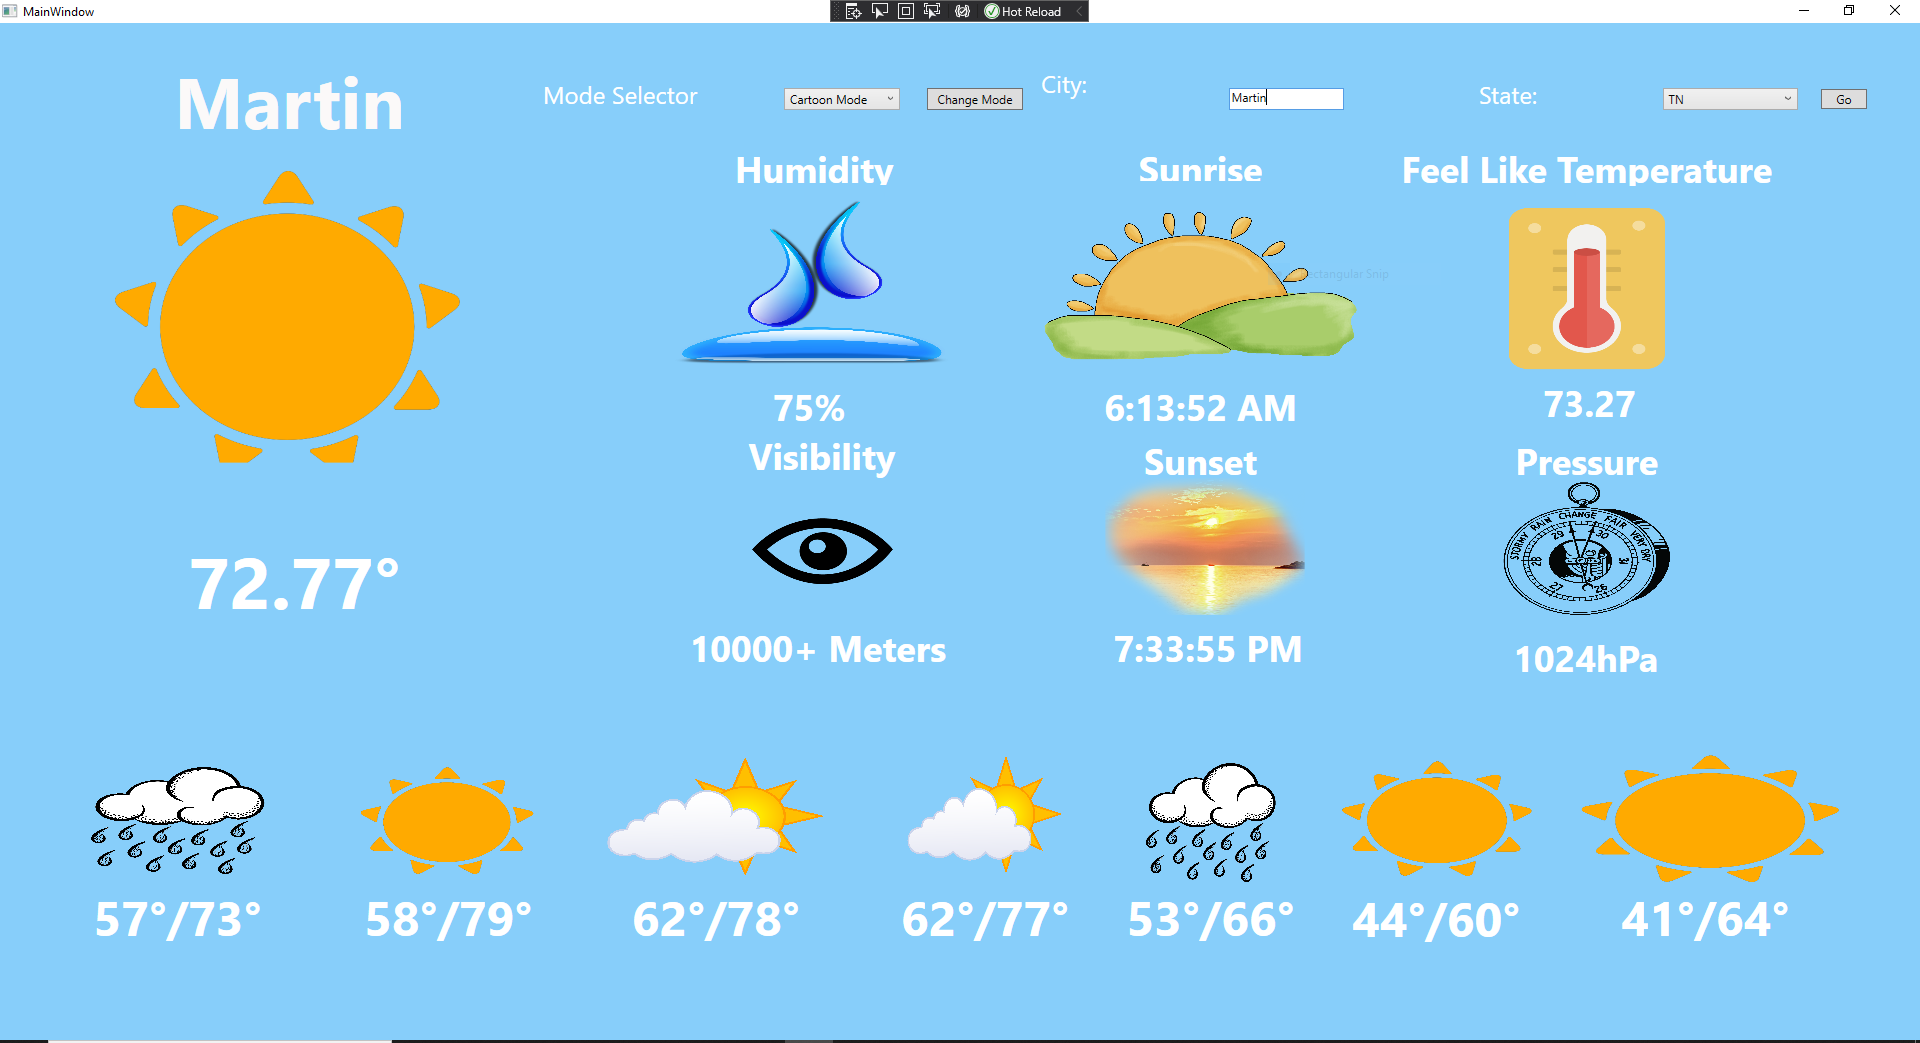
\includegraphics[scale=0.1]{use_case_1.png}
\caption{Illustration of Use Case 1. Here the user has entered a city and state and retrieved the weather information for said location.}
\label{use_case_1}
\end{figure}

\begin{figure}[ht!]
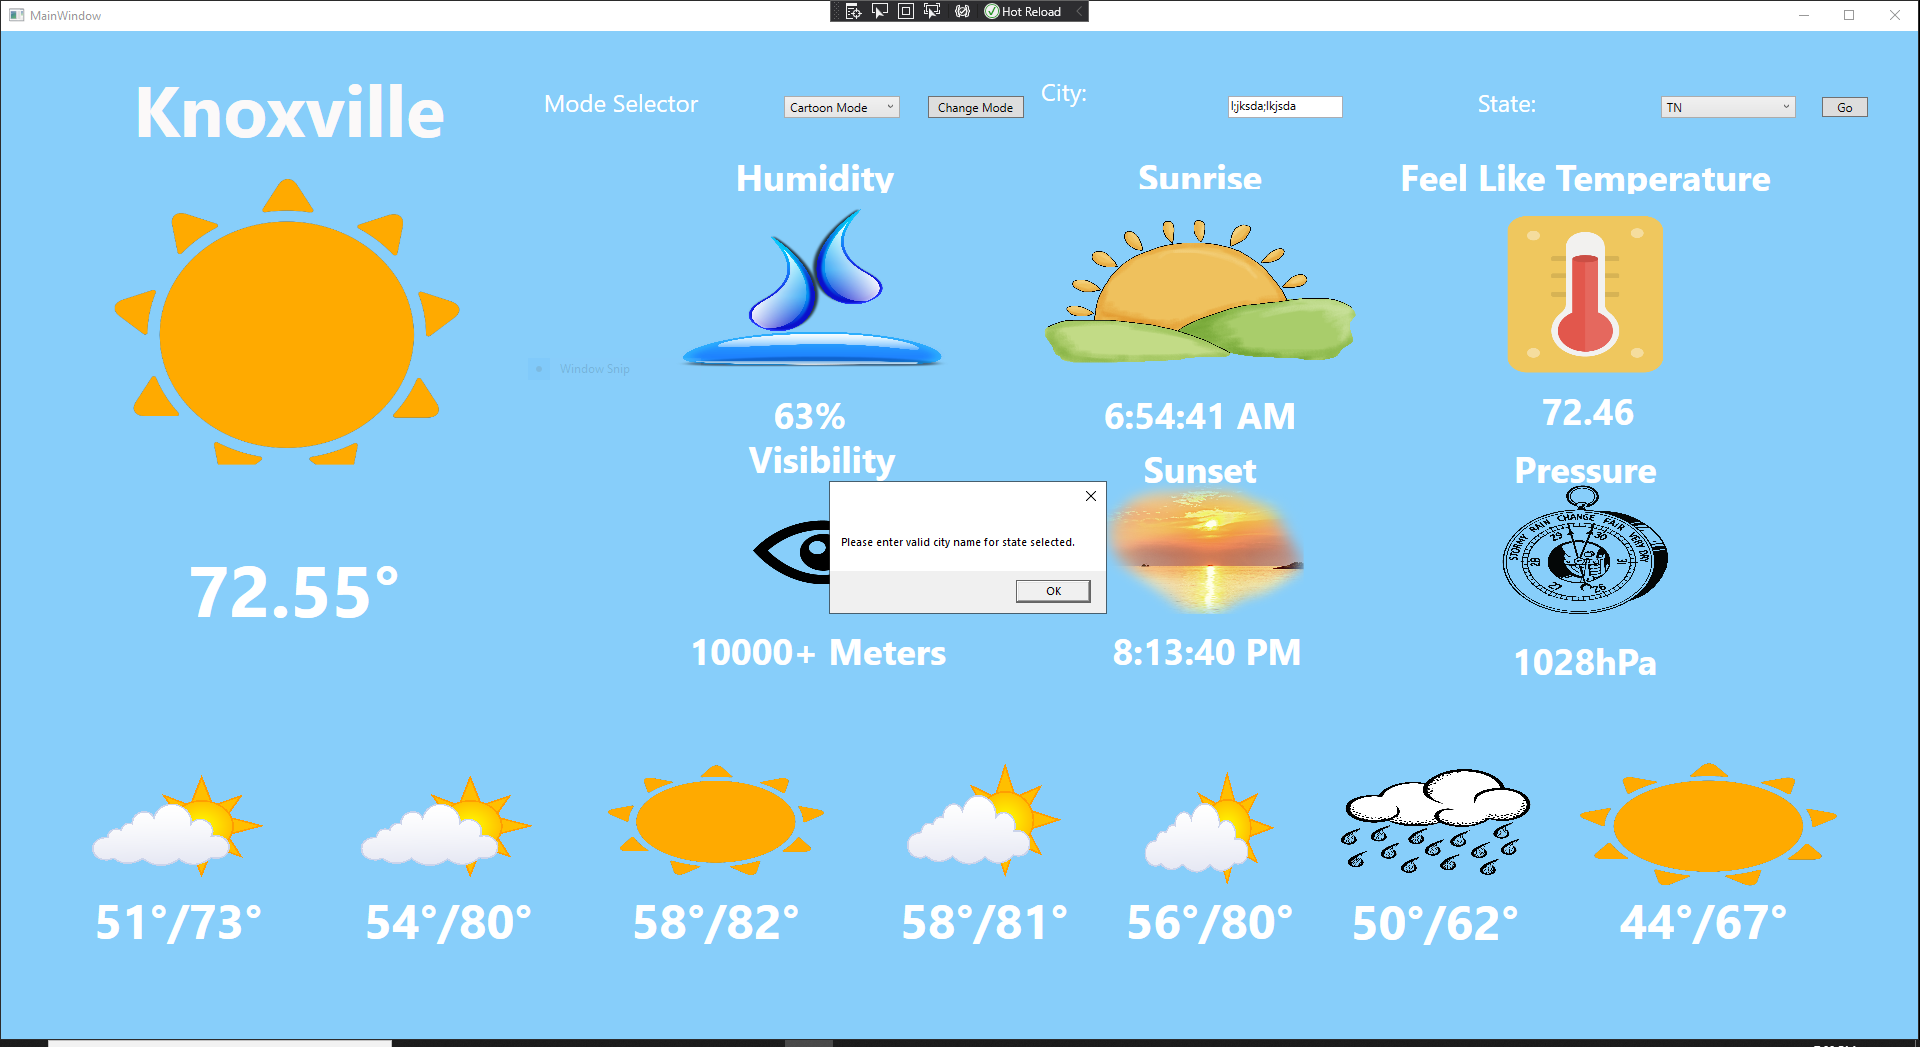
\includegraphics[scale=0.1]{use_case_2.png}
\caption{Illustration of Use Case 2. Here the has entered a city that could not be found in their chosen state.}
\label{use_case_2}
\end{figure}

\begin{figure}[ht!]
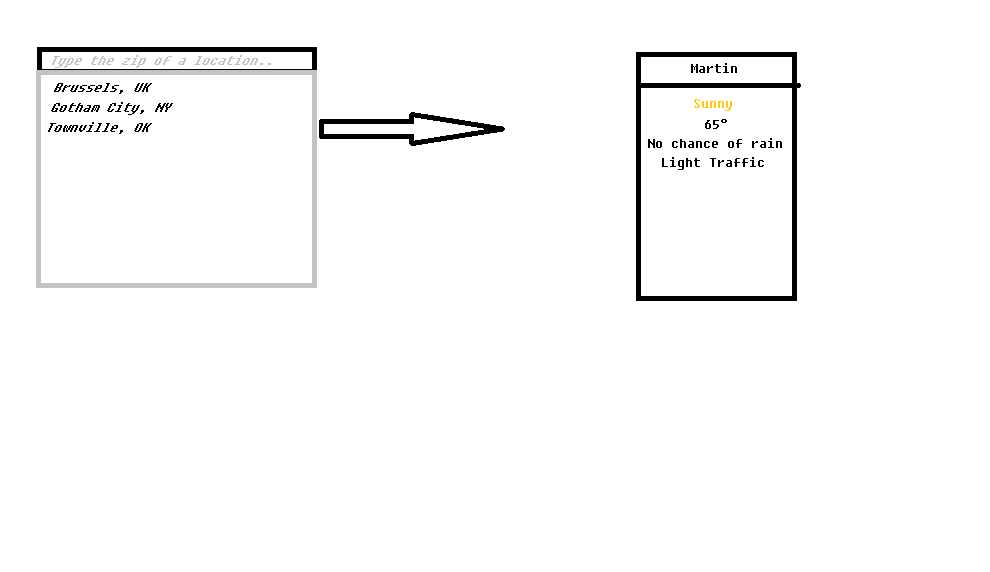
\includegraphics[scale=0.1]{use_case_3.png}
\caption{Illustration of Use Case 3. Here the user has changed the theme.}
\label{use_case_3}
\end{figure}

\subsection{UML Outline}
\begin{figure}[ht!]
\includegraphics[scale = 0.3]{facade_pattern_UltraWeather_modified.png}
\end{figure}

\begin{figure}[ht!]
\includegraphics[scale=0.3]{Singleton_Pattern_UltraWeather.png}
\end{figure}

\section{Project Structure}
The program is structured around the API Container. The Go button acts as a facade for the complex API call that happens once the user enters their city and selects their state. The program uses part of the visitor pattern for themes. All of the data is contained in a temporary City struct that will be destroyed once the data has been given to the relevant fields. This ensures a minimum usage of resources.
The MainWindow class contains the functions for every button and list in our program window, which it uses mainly to access the API Container's call api functions.


\section{Project Timeline}
\begin{figure}[ht !]
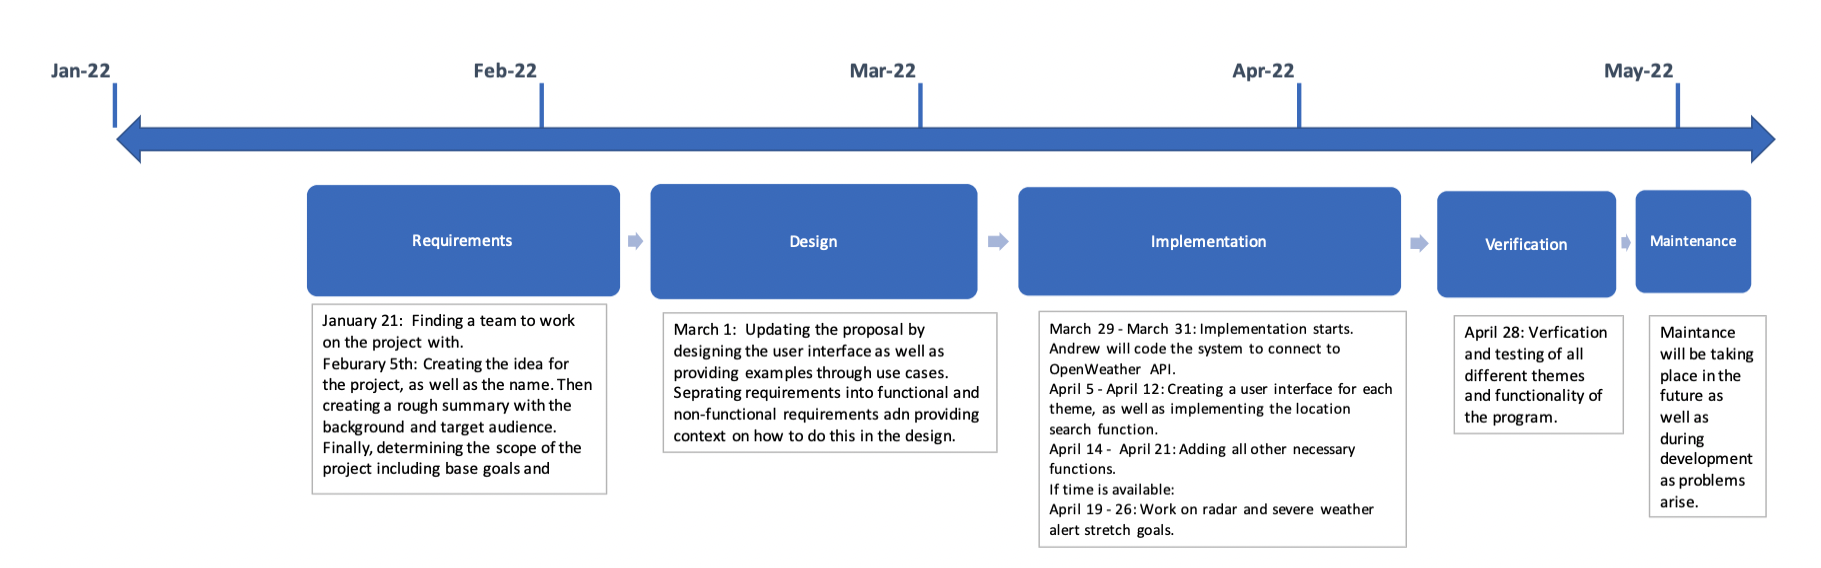
\includegraphics[scale = 0.3]{Timeline.png}
\caption{Full Project Timeline}
\label{TimeLine}
\end{figure}
Milestones:
Feburary 5th: The requirements stage has been discussed and decided.
March 1st: All designs are finished, shown through our use cases.
March 29 - 31: Implementation starts with Andrew coding the system that connects to the API.
April 5 - 12: Implementing the user interface designs shown through the use cases and implementing the location search function.
April 14 - 21: Implementing other functions such as a ForecastPicChangerand functionality for switching modes.
If time is available:
April 19 - 26: Work on radar stretch goal.
April 28: Verfication and testing of all different themes and functionality of the program.
Maintance will be taking place in the future as well as during development as problems arise.



\subsection{Design Patterns Used}
We used a facade pattern and a singleton pattern. The facade pattern comes with the user interface. The user interface is set up in a way that the user can provide information to the system, but they cannot touch anything on the backend. The singleton design pattern was used to make the MainWindow only b initialized once.

\section{Results}
The UltraWeather collects data from OpenWeather API and displays it to the screen in a user friendly way. UltraWeather allows the person to type in a city and checks whether the city is valid. It provides an error MessageBox when it is not valid. The pictures will change when the weather is different, and the forecast will be as accurate as the API.

\subsection{Future Work}
We seek to implement the stretch goals and improve the efficiency of the program even further as our knowledge of computer science grows. Afterwards, we plan to put it on our resumes and forget about the specific details, but keep the knowledge we gained from teh process of finishing the project.


\begin{thebibliography}{1}

\bibitem{IEEEhowto:kopka}
H.~Kopka and P.~W. Daly, \emph{A Guide to \LaTeX}, 3rd~ed.\hskip 1em plus
  0.5em minus 0.4em\relax Harlow, England: Addison-Wesley, 1999.

\end{thebibliography}



\begin{IEEEbiography}{Michael Shell}
Biography text here.
\end{IEEEbiography}

% if you will not have a photo at all:
\begin{IEEEbiographynophoto}{John Doe}
Biography text here.
\end{IEEEbiographynophoto}

% insert where needed to balance the two columns on the last page with
% biographies
%\newpage

\begin{IEEEbiographynophoto}{Jane Doe}
Biography text here.
\end{IEEEbiographynophoto}





% that's all folks
\end{document}

